\vspace*{-6pt}
\section{Discussion and Experiments}\label{sec:discussion}
\vspace*{-4pt}
%Other models to compute contextual embeddings
As detailed in Section~\ref{sec:different-roles}, the ability of the self-attention layers to compute contextual mappings plays a crucial role in the universal approximation property. Interestingly, our analysis shows that replacing the dot-product attention in Transformers with any other component capable of computing contextual mappings should preserve this universal approximation property. This leads naturally to questions about the alternative architectures that realize certain kinds of contextual mappings at different computational and memory costs. 
% Additionally, beyond computing the contextual mappings, what other roles do the attention layers perform?
% Additionally, is the contextual mapping the only role of attention layers, or do they perform other meaningful tasks?
%In Section~\ref{sec:main}, we show that self-attention layers can compute contextual embeddings of input tokens, playing a key role in endowing the Transformer networks with the ability to universally approximate sequence-to-sequence functions. Interestingly, our proof techniques highlight the fact that the property of universal approximation should hold for any architecture that can compute the contextual maps, and subsequently employ the token wise feed-forward maps. This naturally raises some questions, such as, 1) Are there alternate architectures, with different computational and memory requirements, that can implement contextual mapping? 2) In addition to contextual mapping, what are other interesting properties of the functions learned by the self-attention layers?
We explore and discuss some examples of such alternatives in this section.
Our preliminary empirical study demonstrates their practical utility.

%In this section, we will discuss some alternate architectures with the contextual mapping property, thereby also being universal approximators of sequence-to-sequence functions. We then present some preliminary experiments evaluating these architectures.

\vspace*{-5pt}
\subsection{Bi-linear projection}
\vspace*{-3pt}
\label{sec:bi-linear}
Given token embeddings $\mX$ as input, the bi-linear projection layer computes the following update.
\begin{equation*}
%\label{eq:bilinear}
    {\rm BProj}(\mX) = \mX + \mW_O \cdot \mX \cdot \mW_P.
\end{equation*}
The bi-linear projection layer \citep{gong2013learning} is motivated from the ability of random (Gaussian) matrices to map sparse differences to dense vectors~\citep{ailon2009fast}. If there are two input contexts $\mX_1$ and $\mX_2$ that differ in one token, their difference $\mX_1-\mX_2$ is sparse; however, after random projection, the difference $(\mX_1-\mX_2)\mW_P$ will be dense, and the numbers are distinct with high probability, implementing a form ``pair-wise contextual mapping,''\footnote{This guarantee only holds for a finite set (can be exponential in $n$) of fixed vectors in $\reals^n$.} although different from the contextual mapping in Definition~\ref{def:context-mapping}.

%In our experiments we train the matrix $\mW_P$, which means that it is no longer random. We note that after training, bi-linear projection is not a contextual mapping in the strict sense.}.

This layer advantageously incurs smaller number of matrix multiplications as compared to the dot-product attention. That said, the number of parameters in this layer depend on the sequence length, making it harder to reuse the model across tasks with different input sequence lengths. Moreover, the weights used to compute the contextual embeddings ($\mW_P$) are independent of the inputs ($\mX$), whereas in self-attention the weights $(\sfmx [(\mW_K^i \mX)^T \mW_Q^i \mX])$ depend on $\mX$. The first drawback can be addressed by replacing the linear projection with a depth-wise separable convolution layer, which is discussed in the next subsection.

\vspace*{-2pt}
\subsection{Depth-wise separable convolutions}
\vspace*{-3pt}
\label{sec:d-conv}
\begin{figure}[t]
\centering
    \begin{subfigure}[b]{0.48\textwidth}
	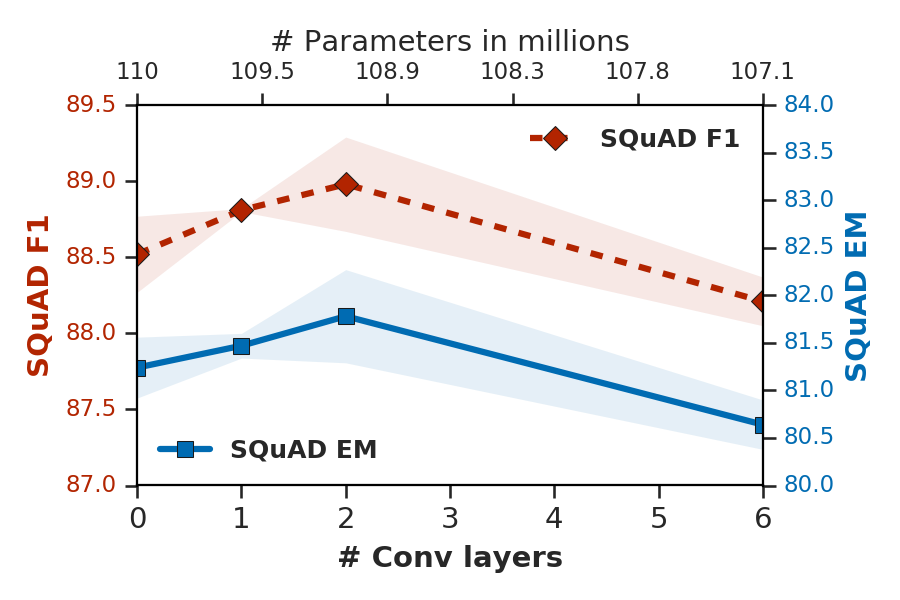
\includegraphics[width=\textwidth]{univ_squad.png}
	\caption{SQuAD}
	\label{fig:squad}
	\end{subfigure}
	\begin{subfigure}[b]{0.48\textwidth}
	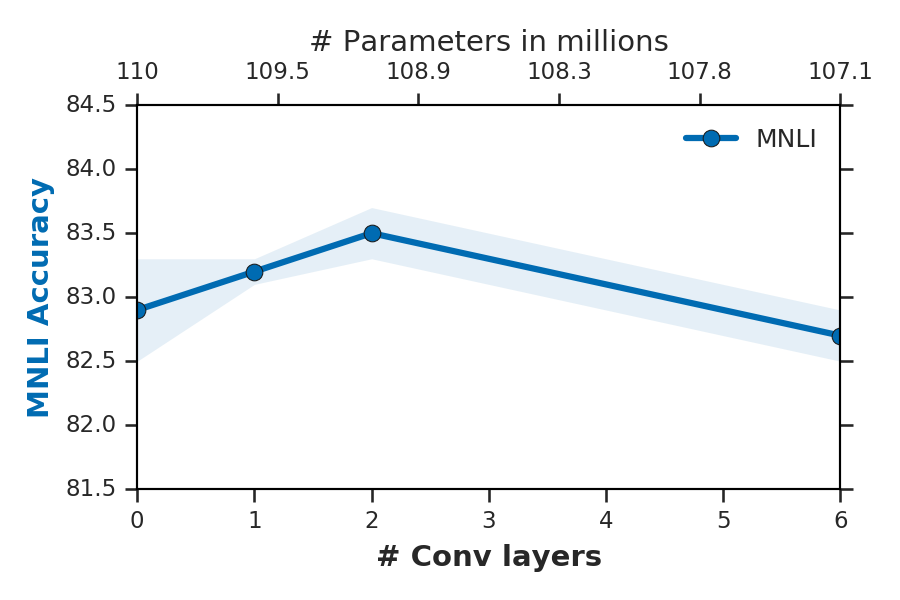
\includegraphics[width=\textwidth]{univ_mnli.png}
	\caption{MNLI}
	\label{fig:mnli}
	\end{subfigure}
	\vspace{-1pt}
	\caption{Performance of hybrid models constructed by first taking $\BB$, a 12 layer Transformer model, and replacing the self-attention layers with depth-wise separable convolution layers, in a varying number of the Transformer blocks closer to the input. Surprisingly, replacing $1$ or $2$ self-attention layers with convolutions improves the performance, while replacing more hurts the performance. This suggests both that Transformers have functionality beyond just computing contextual mappings, and having simpler layers to realize contextual mapping can aid Transformers.}
  \label{fig:conv}
\end{figure}

A depth-wise convolution layer \citep{sifre2014rigid,chollet2017xception,kaiser2017depthwise} involves convolving each dimension of $\mX$ with a corresponding convolution filter of size $k$: \begin{equation*}%\label{eq:conv}
    {\rm SepConv}(\mX) = \mX + \mW_O \left(\mX \ast \mW_C\right),
\end{equation*}
where $\mW_C \in \reals^{d \times k}$ and $\left(\mX \ast \mW_C\right)_{i,:} := \mX_{i,:} \ast (\mW_C)_{i,:}$. Unlike bi-linear projection, this layer can be used across tasks with different input sequence lengths as the number of parameters are independent of the sequence length. While a single layer is unable to compute contextual mappings when the filter size is small, stacking multiple such layers can potentially provide a cheaper way to compute contextual mappings. In fact, based on depth-wise separable convolutions, \citet{wu2019pay} proposed a light-weight dynamic convolution architecture that performs competitively with Transformers on machine translation. 

%%%%%%%%%%%%%%%%%%%%%%%%%%%%%%%%%%%%%%%%%%%%%%%%%%%%%%%

\vspace*{-5pt}
\subsection{Experiments}
\vspace*{-3pt}

We now present our experiments with these other architectures, with the goal of understanding the extent to which computing contextual mappings can capture the performance of Transformers. As discussed earlier, ${\rm BProj}$ and ${\rm SepConv}$ do \emph{not} implement contextual mappings (cf.~Definition~\ref{def:context-mapping}), so we do not expect that either ${\rm BProj}$ or ${\rm SepConv}$ based models to have the same performance as the expensive Transformers. These models do not use input dependent weights to compute attention, and hence have weaker representation power. Instead, our goal is to see if we can use these cheaper layers to replace (some of) the expensive self-attention layers.

%We now empirically compare ${\rm BProj}$ and ${\rm SepConv}$ based models to Transformers on two NLP tasks. As argued in Section~\ref{sec:bi-linear} and \ref{sec:d-conv}, these seemingly weaker models can indeed realize the contextual mappings up to a certain extent. Thus, our experiments are geared towards exploring if the performance of Transformers can be solely attributed to the contextual mappings.


We follow the experimental setting from \citet{devlin2018bert} to train the Transformers, with the masked language model pre-training followed by a task specific fine-tuning, and work with a $12$ layer architecture based on $\BB$. We present our results on a question answering task (SQuAD) \citep{rajpurkar2016squad} and a sentence entailment task (MNLI) \citep{mnli}. In our first set of experiments we train models that employ ${\rm BProj}$ and ${\rm SepConv}$ layers, instead of the self-attention layer in eq.\eqref{eq:attn}. We notice that, as expected, these simpler models have weaker performance than the self-attention layer. See Table \ref{table:large_batch} in Section \ref{sec:appx_experiments} for a comparison of these models on MNLI. 

%of the original 12 layer Transformer model \footnote{Here, we use a batch size of 8k, different from the small batch setup in Fig.~\ref{fig:conv} and \citep{devlin2018bert}}. \todo{Add a table in the appendix.}


%At a first glance, both these models look much weaker than self-attention models. However as we discussed earlier, even these simpler models can compute contextual embeddings, albeit with weights that are independent of the input. Hence, experimentally comparing them with Transformers can suggest how much of  the performance of the transformers is due to their ability to compute contextual embeddings. 

%We experimentally compare these models to Transformers, to see the importance of contextual embedding property for two NLP tasks. The goal of our experiments is only to verify the sufficiency of architectures having contextual embedding property. We chose the  two stage setup from \citep{devlin2018bert}, with masked language model pre-training followed by task specific fine-tuning. We work with a 12 layer architecture based on $\BB$. In our first set of experiments we train models that employ Bi-linear projection layers~(cf.~\eqref{eq:bilinear}) and the depth-wise convolution layers~(cf.~\eqref{eq:conv}), instead of the self attention layers in Transformers~(cf.~\eqref{eq:attn}). We notice that even these simple models perform reasonably well, with MNLI accuracies of $72.3\%$ and $73\%$ respectively, compared to $78.2\%$ of the original 12 layer Transformer model \footnote{These are experiments with a batch size of 8k, different from the small batch setting results in Figure~\ref{fig:conv} and \citep{devlin2018bert}}. \todo{Add a table in the appendix.}

Next, we swap a varying number of the first few self-attention layers in $\BB$ with ${\rm SepConv}$, implemented with filter reuse across dimensions \citep{wu2019pay}\footnote{We refer to Section \ref{sec:appx_experiments} for a complete description of the setup.}. Fig.~\ref{fig:conv} illustrates the performance of these hybrid models.  Interestingly, models with $1$ or $2$ convolution layers and rest the self-attention layers, perform better than models with only the self-attention layers.
Note that, replacing self-attention layer with ${\rm SepConv}$ also reduces the computational cost and the number of parameters. 
One explanation we have is that the first few attention layers tend to attend broadly to the whole sequence (as empirically observed in \citep{clark2019does}), and the cheaper convolution layers can perform this job more efficiently. A detailed evaluation of such hybrid architectures will be interesting future research.
%This suggests that, having cheaper convolution layers can aid the Transformer, by potentially computing the contextual mappings efficiently. 

%This we hypothesize could be due \todo{...}
%The model with only convolution layers is consistently inferior to Transformers, as we noticed earlier.

Our experiments also call for a deeper understanding of the exact nature of the embeddings computed by practical attention models.
Since Transformers in practice have fixed depth, we believe that they might not be able to exactly implement contextual mappings as we defined in Definition~\ref{def:context-mapping}. 
However, there is some preliminary empirical evidence that Transformers do implement some sort of ``contextual mappings.'' For example,
Fig.~4 of \citet{coenen2019visualizing} presents visualizations of
embeddings of a single word in different contexts (sentences). They experimentally notice that Transformers, in addition to computing contextual mappings, also map a word into semantic clusters. Formalizing and evaluating this property of Transformers is an interesting direction for future work. We again note that \citet{wu2019pay} have proposed an alternative way to compute such embeddings based on dynamic convolution layers. Evaluating the mappings computed by these models should shed more light on the workings of attention models and inspire efficient and better performing architectures.

